
\chapter{Simulations}\label{chapter:simulations}

In this chapter I want to give an intuition for the results on \textit{no-regret} convergence in finite games discussed in chapter \ref{chapter:literatureReview}. I have implemented both, \textit{Online Gradient Ascent with Lazy Projections} (OGALP) and \textit{Normalized Exponentiated Gradient} (NEG). As expected both algorithms show very similar behavior. The \textit{steep entropic regularizer} used in NEG slightly reshaped space in comparison to the common \textit{Euclidean regularizer} in OGALP. In terms of convergence, however, both behave identically. For that reason, I might show plots of only one algorithm.  I found converge in frequency of play in constant sum games I have limited myself on 2x2 and 3x3 matrix games as higher dimensional games are hard to illustrate. Therefore we have $\mathcal{N} = \{1,2\}$ throughout this chapter. As already mentioned the outcome of \textit{no-regret} learning depends on the type of game and the type of eqilibria. The chapter is structured accordingly. 

\section{Unique Mixed Nash Equilibrium}\label{section:uniqueMixedNashEquilibrium}

\subsection{Matching Pennies}\label{subsection:machtingPennies}

\begin{itemize}
    \item More specifically, regardless of the choice of the initial
condition there are only a finite number of iterations where both players select mixed strategies (show single trajectory)
\end{itemize}

Matching Pennies is a simple two player zero sum game. Both player choose between \textit{Heads} and \textit{Tails} and if they match then the \textit{row player} wins and if they mismatch the \textit{column player} wins. The payoff is set accordingly as in \ref{tab:payoffMachtingPennies}. 

\begin{table}[H]\centering
\setlength{\extrarowheight}{2pt}
\begin{tabular}{cc|c|c|}
  & \multicolumn{1}{c}{} & \multicolumn{1}{c}{$Heads$}  & \multicolumn{1}{c}{$Tails$} \\\cline{3-4}
  & $Heads$ & $1,-1$ & $-1,1$ \\\cline{3-4}
  & $Tails$ & $-1,1$ & $1,-1$ \\\cline{3-4}
\end{tabular}\caption{\label{tab:payoffMachtingPennies}payoff matrix Matching Pennies}
\end{table}

There is only a single \textit{fully mixed Nash equilibrium} (MNE), i.e. when both players chooses \textit{Heads} and \textit{Tails} equally likely. 

\begin{equation*}
    x_{i}^{*} = (1/2,1/2) \qquad \forall i \in \mathcal{N}
\end{equation*}

As stated in proposition \ref{prop:noInteriorStable} no \textit{fully mixed strategy}, and therefore no \textit{fully mixed Nash equilibrium}, can be stable under FoReL algorithms. Since FoReL can only converge to \textit{stable} states or \textit{strict Nash Equilibira} equivalently (see proposition \ref{prop:StrictStableEquivalent}), for both NEG and OGALP the induced sequence of play fail to converge. In fact both exhibit finite cyclic behaviour around the unique MNE as illustrated in the figures \ref{fig:Pennies1} and \ref{fig:Pennies2}. Note that \textit{P(Tails)} is implicitly given by $1 -$\textit{P(Heads)}. 

\begin{figure}[H]
    \centering
    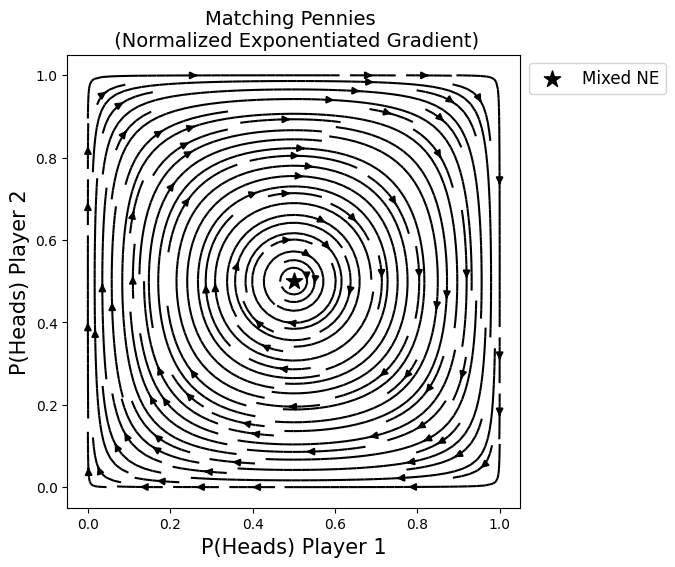
\includegraphics[width=0.5\textwidth]{logos/Pennies1.png}
    \caption{NEG vector field in Matching Pennies}
    \label{fig:Pennies1}
\end{figure}

\begin{figure}[H]
    \centering
    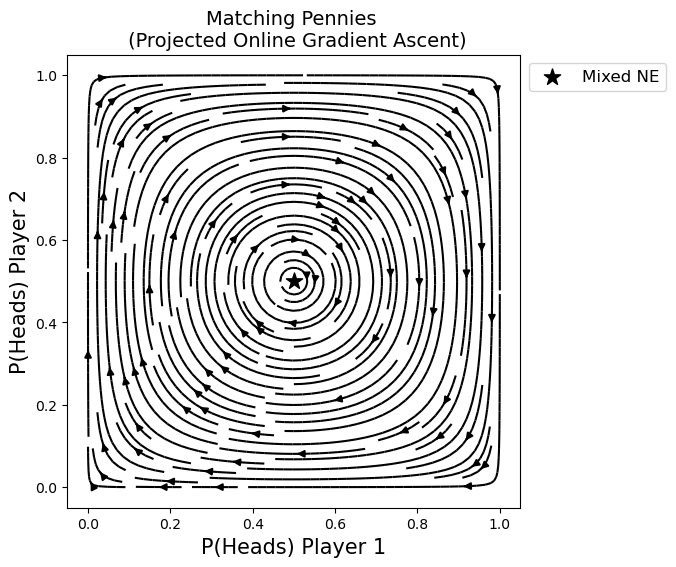
\includegraphics[width=0.5\textwidth]{logos/Pennies2.png}
    \caption{OGALP vector field in Matching Pennies}
    \label{fig:Pennies2}
\end{figure}

Interestingly, the empirical frequency of play, however, ultimately converges to the unique MNE. That happened independently from the initial strategies of the players. The amplitude of of cycles dampens over time as in figure \ref{fig:Pennies3}.

\begin{figure}[H]
    \centering
    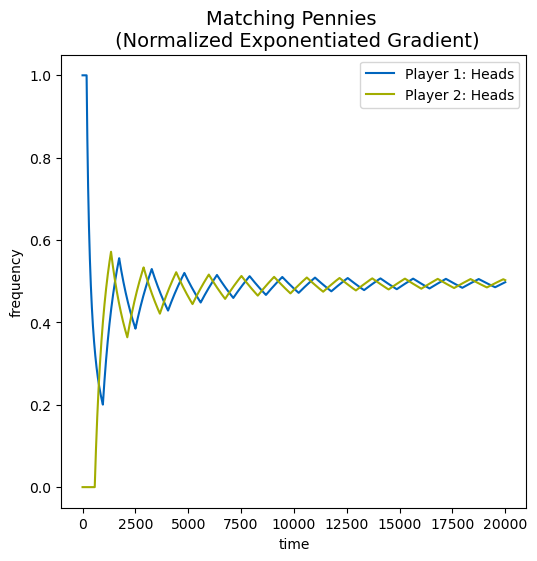
\includegraphics[width=0.5\textwidth]{logos/Pennies3.png}
    \caption{NEG empirical frequency of play in Matching Pennies}
    \label{fig:Pennies3}
\end{figure}

An explanation for the convergence behavior in Matching Pennies could be its zero sum property. I have slightly adjusted the payoff matrix such that we don't have zero sum but constant sum. 

\begin{table}[H]\centering
\setlength{\extrarowheight}{2pt}
\begin{tabular}{cc|c|c|}
  & \multicolumn{1}{c}{} & \multicolumn{1}{c}{$Heads$}  & \multicolumn{1}{c}{$Tails$} \\\cline{3-4}
  & $Heads$ & $1,0$ & $0,1$ \\\cline{3-4}
  & $Tails$ & $0,1$ & $1,0$ \\\cline{3-4}
\end{tabular}\caption{\label{tab:payoffNonZeroMachtingPennies}payoff matrix Non Zero Matching Pennies}
\end{table}

Note that this version yield the same unique \textit{fully mixed Nash equilibrium} as in the zero sum version where both players choose \textit{Heads} and \textit{Tails} equally likely. Interestingly, the behavior of both algorithms has not changed at all. I still find convergence in frequencies to the MNE as in figure \ref{fig:Pennies3}. Also the  cyclic trajectories as described in figure \ref{fig:Pennies1} and \ref{fig:Pennies2} were exactly the same for the constant sum version. Therefore we can conclude that the convergent behavior is not justified by the games zero sum property.


\subsection{Rock Paper Scissors}\label{subsection:rockPaperScissors}

One might think the convergence of empirical frequencies to the game's MNE is an artifact of its simple 2x2 structure, but I found similar behavior in Rock Paper Scissors, another constant-sum game.

\begin{table}[H]\centering
\setlength{\extrarowheight}{2pt}
\begin{tabular}{cc|c|c|c|}
  & \multicolumn{1}{c}{} & \multicolumn{1}{c}{$Rock$}  & \multicolumn{1}{c}{$Paper$}  & \multicolumn{1}{c}{$Scissors$} \\\cline{3-5}
            & $Rock$ & $0,0$ & $-1,1$ & $1,-1$ \\ \cline{3-5}
            & $Paper$ & $1,-1$ & $0,0$ & $-1,1$ \\\cline{3-5}
            & $Scissors$ & $-1,1$ & $1,-1$ & $0,0$ \\\cline{3-5}
\end{tabular}\caption{\label{tab:payoffRPS}payoff matrix Rock Paper Scissors}
\end{table}

The only \textit{Nash equilibrium} that exists is the following \textit{fully mixed} NE

\begin{equation*}
    x_{i}^{*} = (1/3,1/3,1/3) \qquad \forall i \in \mathcal{N}
\end{equation*}

After roughly $50$ timesteps, both algorithms exhibit finite out-of-sync cyclic behavior as shown in figure \ref{fig:RPS2}. The players essentially chase one another. Note that the initial strategies are set randomly. 

\begin{figure}[H]
    \centering
    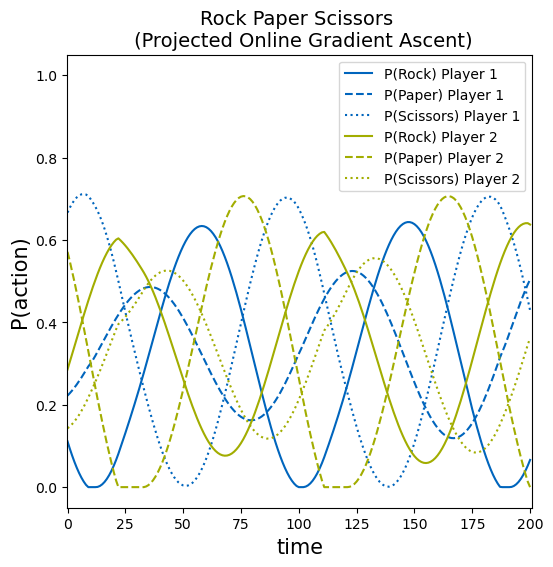
\includegraphics[width=0.5\textwidth]{logos/RPS2.png}
    \caption{OGALP weights in Rock Paper Scissors}
    \label{fig:RPS2}
\end{figure}


Again, the empirical frequencies, on the other hand, converge to the game's unique MNE as in figure \ref{fig:RPS3}

\begin{figure}[H]
    \centering
    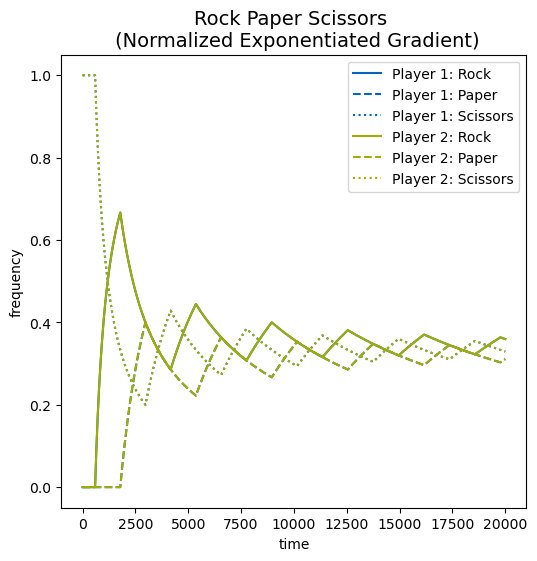
\includegraphics[width=0.5\textwidth]{logos/RPS3.png}
    \caption{NEG empirical frequency of play in Rock Paper Scissors}
    \label{fig:RPS3}
\end{figure}


\subsection{Shapley Game}\label{subsection:shapleyGame}

The Shapley Game resembles that of Rock Paper Scissors. But Shapley is not constant-sum but general-sum. In the payoff matrix in \ref{tab:payoffShapley} we can see that the utility of an action profile sometimes sums up to $1$ and sometimes to $0$. 

\begin{table}[H]\centering
\setlength{\extrarowheight}{2pt}
\begin{tabular}{cc|c|c|c|}
  & \multicolumn{1}{c}{} & \multicolumn{1}{c}{$L$}  & \multicolumn{1}{c}{$C$}  & \multicolumn{1}{c}{$R$} \\\cline{3-5}
            & $T$ & $1,0$ & $0,1$ & $0,0$ \\ \cline{3-5}
            & $M$ & $0,0$ & $1,0$ & $0,1$ \\\cline{3-5}
            & $B$ & $0,1$ & $0,0$ & $1,0$ \\\cline{3-5}
\end{tabular}\caption{\label{tab:payoffShapley}payoff matrix Shapley Game}
\end{table}

The game's unique NE is the same \textit{fully mixed Nash equilibrium} as in Rock Paper Scissors

\begin{equation*}
    x_{i}^{*} = (1/3,1/3,1/3) \qquad \forall i \in \mathcal{N}
\end{equation*}

In this case, both NEG and OGALP, are non convergent neither in weights nor in frequencies. Again the weights cycle through the space of possible strategies but this time the cycles grow exponentially, see figure \ref{fig:Shapley1}. As far as frequencies are concerned the amplitudes of the cycles do not dampen over time (Fig. \ref{fig:Shapley2}) as it did in Matching Pennies or Rock Paper Scissors. They rather cycle exponentially again. Similar results are shown in \cite{jafari}. They suggest that the convergence of frequencies to the game's MNE is because of its constant sum structure. In general sum games, like the Shapley Game, \textit{no regrets} dynamics fail to converge. The same behaviour was found for \textit{fictitious play}, a simple \textit{best response} dynamic that is not a \textit{no regret} algorithm \cite{jafari}.

\begin{figure}[H]
    \centering
    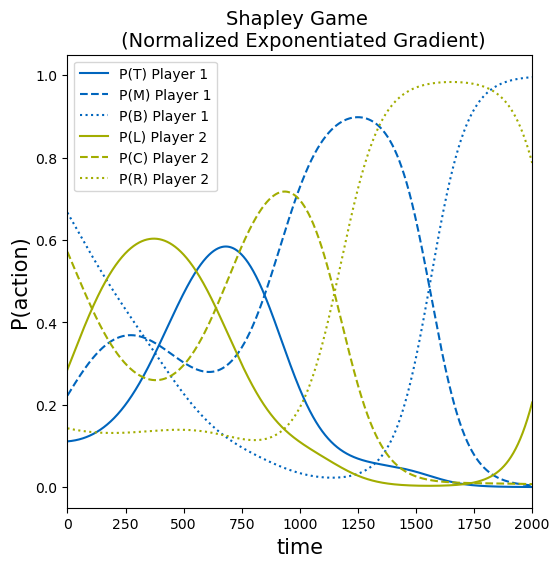
\includegraphics[width=0.5\textwidth]{logos/Shapley1.png}
    \caption{NEG weights in the Shapley Game}
    \label{fig:Shapley1}
\end{figure}

\begin{figure}[H]
    \centering
    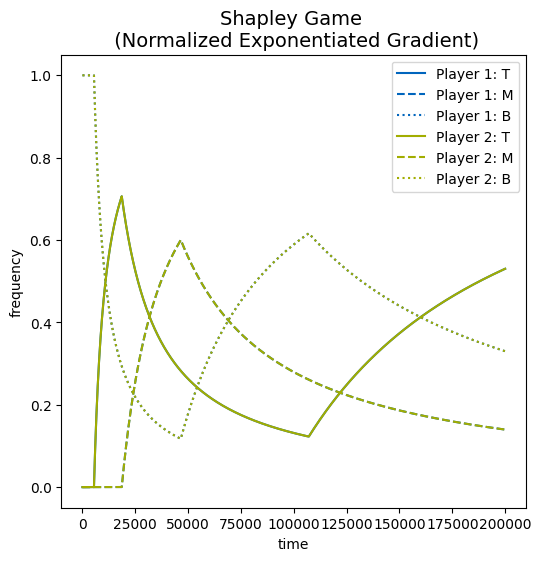
\includegraphics[width=0.5\textwidth]{logos/Shapley2.png}
    \caption{NEG empirical frequency of play in the Shapley Game}
    \label{fig:Shapley2}
\end{figure}



\section{Unique Pure Nash Equilibrium}\label{section:uniquePureNashEquilibrium}

\subsection{Prisoner's Dilemma}\label{subsection:prisonersDilemma}

The next game I would like to address is the famous Prisoner's Dilemma. The game works as follows. Two bank robbers have been arrested. They are separated from each other and both can choose either to stay silent or to betray the other one by admitting the crime. When both stay silent, both are sent to prison for only one year. When both betray they go to jail for 2 years each. However, if one stays silent while the other betrays the one that stayed silent goes is sent to prison for 3 years while the other one is set free, see table \ref{tab:payoffPrisoners}.

\begin{table}[H]\centering
\setlength{\extrarowheight}{2pt}
\begin{tabular}{cc|c|c|}
  & \multicolumn{1}{c}{} & \multicolumn{1}{c}{$Silent$}  & \multicolumn{1}{c}{$Betray$} \\\cline{3-4}
  & $Silent$ & $-1,-1$ & $-3,0$ \\\cline{3-4}
  & $Betray$ & $0,-3$ & $-2,-2$ \\\cline{3-4}
\end{tabular}\caption{\label{tab:payoffPrisoners}payoff matrix Prisoner's Dilemma}
\end{table}

The only \textit{Nash equilibrium} is when both players always choose \textit{Betray}. So there is no \textit{fully mixed Nash equilibrium} but only one \textit{pure Nash equilibrium}. 

\begin{equation*}
    x^{*} = (Betray,Betray) \qquad \textit{strict }\text{PNE}
\end{equation*}

Note that the PNE is also \textit{strict}. Any unilateral deviation from the PNE would lead to a reduction in payoff. For instance, if the \textit{row player} knows that the \textit{column player}  chooses \textit{Betray} then deviating from \textit{Betray} would decrease the \textit{row player's} payoff, from $-2$ to $-3$. As the game is symmetric the same holds for the \textit{column player}. \\

The blue region in figure \ref{fig:Prisoners2} indicates strategies that are \textit{stable} with respect to the PNE in a sense of definition \ref{def:stability}. As we can see the PNE is \textit{globally stable}. As stated in proposition \ref{prop:globalConvergence} \textit{no-regret} dynamics converge globally to the \textit{globally stable equilibrium}. As the vector field in the same figure \ref{fig:Prisoners2} suggests, NEG indeed converges globally to the games's unique PNE. We have the same result for OGDLP, see figure \ref{fig:Prisoners3}.

\begin{figure}[H]
    \centering
    \captionsetup{justification=centering}
    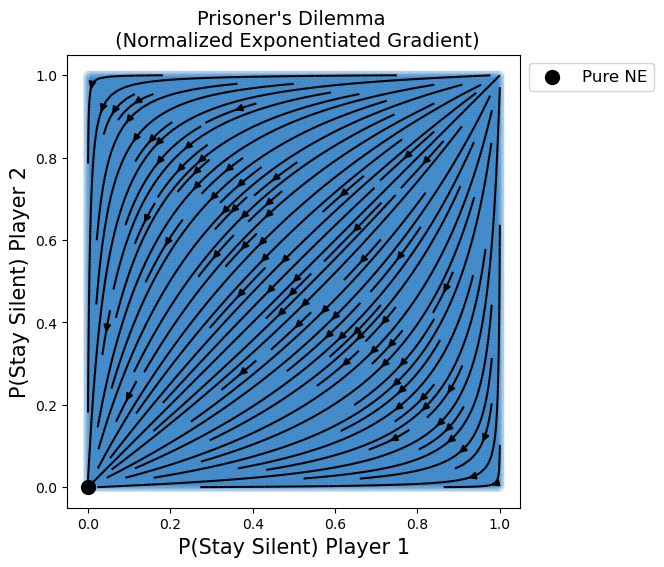
\includegraphics[width=0.5\textwidth]{logos/Prisoners2.png}
    \caption{NEG vector field in Prisoner's Dilemma. Stable region with respect to the PNE is colored in blue}
    \label{fig:Prisoners2}
\end{figure}

\begin{figure}[H]
    \centering
    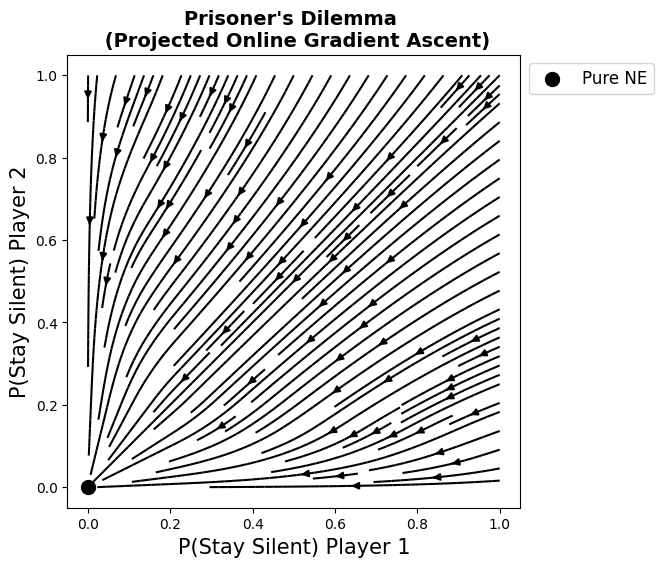
\includegraphics[width=0.5\textwidth]{logos/Prisoners3.png}
    \caption{OGDLP vector field in Prisoner's Dilemma}
    \label{fig:Prisoners3}
\end{figure}

\section{Mixed and Pure Nash Equilibria}\label{section:MixedandPureNashEquilibria}

\subsection{Battle Of Sexes}\label{subsection:battleOfSexes}

Image a couple of two persons with different interests. One would prefer to watch a boxing fight, say the \textit{row player}, and the other one prefers to go to a ballet, the \textit{column player}. But they would rather spend time together than choosing different events. There is no communication between both. The payoff is set accordingly as in table \ref{tab:payoffBattleOfSexes}.

\begin{table}[H]\centering
\setlength{\extrarowheight}{2pt}
\begin{tabular}{cc|c|c|}
  & \multicolumn{1}{c}{} & \multicolumn{1}{c}{$Fight$}  & \multicolumn{1}{c}{$Ballet$} \\\cline{3-4}
  & $Fight$ & $3,2$ & $0,0$ \\\cline{3-4}
  & $Ballet$ & $0,0$ & $2,3$ \\\cline{3-4}
\end{tabular}\caption{\label{tab:payoffBattleOfSexes}payoff matrix Battle of Sexes}
\end{table}

There are two quite obvious \textit{pure Nash equilibria}. One where both choose \textit{Fight}, and one where both choose \textit{Ballet}. But there is also a \textit{fully mixed Nash equilibrium}, i.e when both players randomize over the actions. In particular the \textit{row player} should choose \textit{Fight} with probability $2/3$ and \textit{Ballet} with $1/3$ and the \textit{column player} should choose \textit{Fight} with $1/3$ and \textit{Ballet} with $2/3$. In formulas we have the following \textit{Nash equilibria}

\begin{description}\centering
    \item $x^{*} = (Fight,Fight) \qquad \textit{strict }\text{PNE}$
    \item $x^{*} = (Betray,Betray) \qquad \textit{strict }\text{PNE}$
    \item $x_{1}^* = (2/3,1/3) \qquad x_{2}^* = (1/3,2/3) \qquad \text{MNE}$
\end{description}

Note that again both PNEs are \textit{strict} in a sense of definition \ref{def:strictNE}. Neither the \textit{row player} nor the \textit{column player} can unilaterally deviate from an PNE without reducing its payoff. According to proposition \ref{prop:StrictStableEquivalent} that means both PNE are also \textit{stable} states as defined in \ref{def:stability}. Then both PNEs must also be locally attracting (proposition \ref{prop:localConvergence}). And indeed, as shown in figure \ref{fig:BattleOfSexes5}, the NEG algorithm converges locally to the corresponding PNE. Notice how the stable regions of the PNEs intersect. 

\begin{figure}[H]
    \centering
    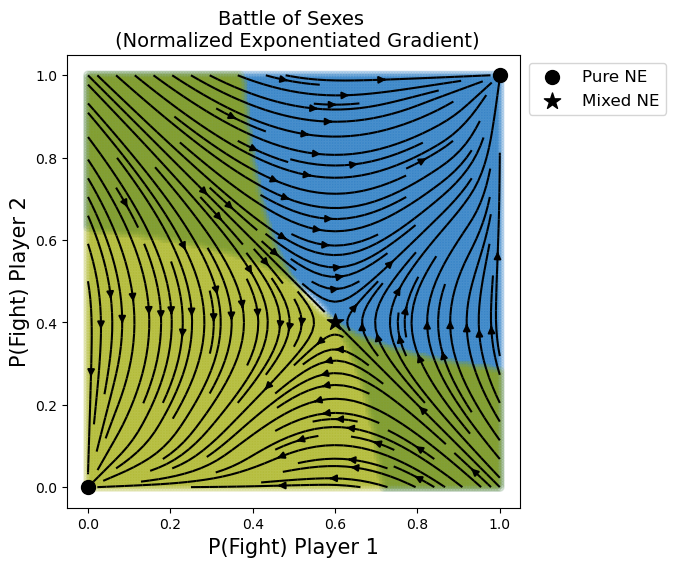
\includegraphics[width=0.5\textwidth]{logos/BattleOfSexes5.png}
    \caption{NEG vector field in Battle of Sexes with stable regions for both PNEs}
    \label{fig:BattleOfSexes5}
\end{figure}

For clarification I have highlighted only the stable region with respect to the PNE \textit{(Fight,Fight)} in figure \ref{fig:BattleOfSexes2}. Also notice that not all points in the stable region converge to the corresponding PNE. In this game, for instance, all initial point above the diagonal between \textit{(Fight,Ballet)} and \textit{(Ballet,Fight)} converge to the PNE \textit{(Fight,Fight)} and all point below converge to the PNE \textit{(Ballet,Ballet)}. 

\begin{figure}[H]
    \centering
    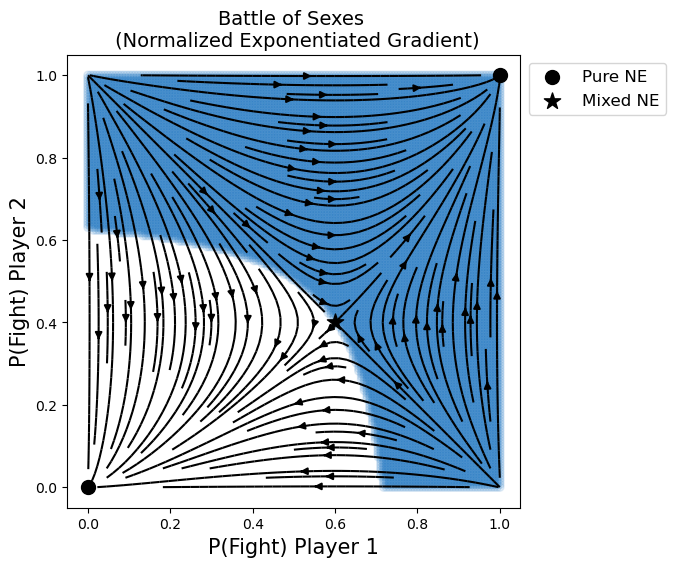
\includegraphics[width=0.5\textwidth]{logos/BattleOfSexes2.png}
    \caption{NEG vector field in Battle of Sexes with stable regions for the PNE \textit{(Fight,Fight)}}
    \label{fig:BattleOfSexes2}
\end{figure}

The question might raise whether the MNE can be \textit{stable} as well. Even though there is a stable region for the MNE as depicted in \ref{fig:BattleOfSexes3}, we cannot find a neighborhood for the MNE such that the inequality of the stability definition (\ref{def:stability}) holds. Intuitively, no matter how far we zoom in to the MNE we cannot draw a circle around it such that all points within the circle are blue as illustrated in figure \ref{fig:BattleOfSexes4}. Therefore except from the perfect diagonal between \textit{(Fight,Ballet)} and \textit{(Ballet,Fight)} the algorithms never converges towards the MNE. That is align with proposition \ref{prop:noInteriorStable} that no interior point can be \textit{stable} under FoReL.  

\begin{figure}[H]
    \centering
    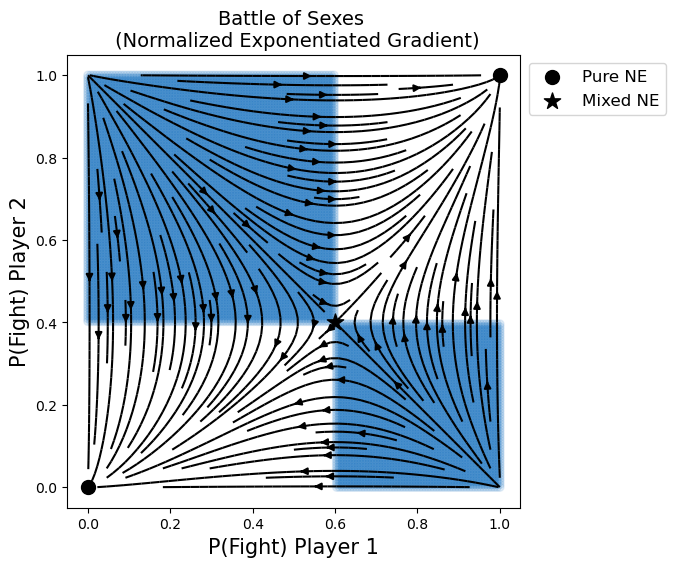
\includegraphics[width=0.5\textwidth]{logos/BattleOfSexes3.png}
    \caption{Stable region for MNE in Battle of Sexes}
    \label{fig:BattleOfSexes3}
\end{figure}

\begin{figure}[H]
    \centering
    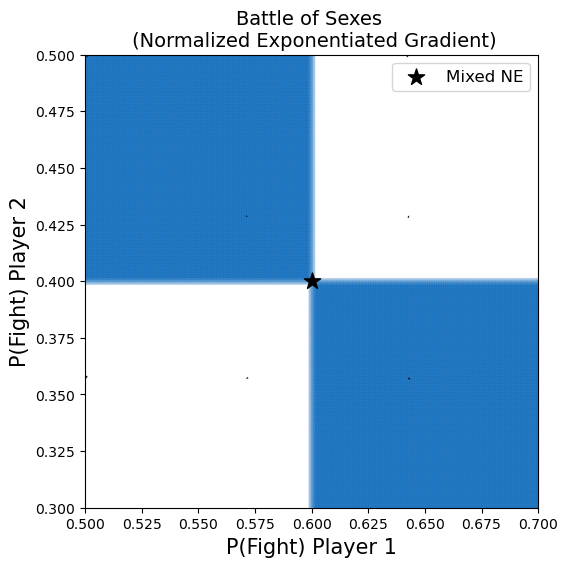
\includegraphics[width=0.5\textwidth]{logos/BattleOfSexes4.png}
    \caption{Zoomed in to the MNE in Battle of Sexes}
    \label{fig:BattleOfSexes4}
\end{figure}


\subsection{Intersection Game}\label{subsection:intersectionGame}

Lets revisit the intersection game from subsection \ref{subsection:CEandCCE}. The game involves two car drivers that need to cross an intersection without a crash. They can either \textit{Stop} or \textit{Go}. The driver's payoff is straight forward as in table \ref{tab:payoffIntersection}. 

\begin{table}[H]\centering
\setlength{\extrarowheight}{2pt}
\begin{tabular}{cc|c|c|}
  & \multicolumn{1}{c}{} & \multicolumn{1}{c}{$Stop$}  & \multicolumn{1}{c}{$Go$} \\\cline{3-4}
  & $Stop$ & $0,0$ & $0,1$ \\\cline{3-4}
  & $Go$ & $1,0$ & $-100,-100$ \\\cline{3-4}
\end{tabular}\caption{\label{tab:payoffIntersection}payoff matrix Intersection Game}
\end{table}

Similar to the Battle of Sexes the game has two \textit{pure Nash equilibria}, namely \textit{(Stop, Stop)} and \textit{(Go,Go)}, and a single \textit{mixed Nash equilibrium} where both drivers choose to \textit{Stop} with probability $100/101$ and \textit{Go} with probability $1/101$. To sum up we have the following \textit{Nash equilibria}.

\begin{description}\centering
    \item $x^{*} = (Go,Go) \qquad \textit{strict }\text{PNE}$
    \item $x^{*} = (Stop,Stop) \qquad \textit{strict }\text{PNE}$
    \item $x_{1}^* = x_{2}^* = (100/101,1/101) \qquad \text{MNE}$
\end{description}

Again it is easy to check that both PNEs are also \textit{strict} and therefore \textit{stable} states (proposition \ref{prop:StrictStableEquivalent}). I have colored the \textit{stable} regions for both PNEs. We can see that both PNEs are indeed \textit{locally stable} states. Just like stated in proposition \ref{prop:localConvergence} our \textit{no-regret} algorithms therefore need to locally converge to the PNEs. In fact both algorithms converge to the PNE that is the "closest" one from the initial strategy just like in Battle of Sexes, see figure \ref{fig:Intersection4}. Note that the MNE denoted by the star is indeed a \textit{fully mixed} NE even though it looks like a PNE.

\begin{figure}[H]
    \centering
    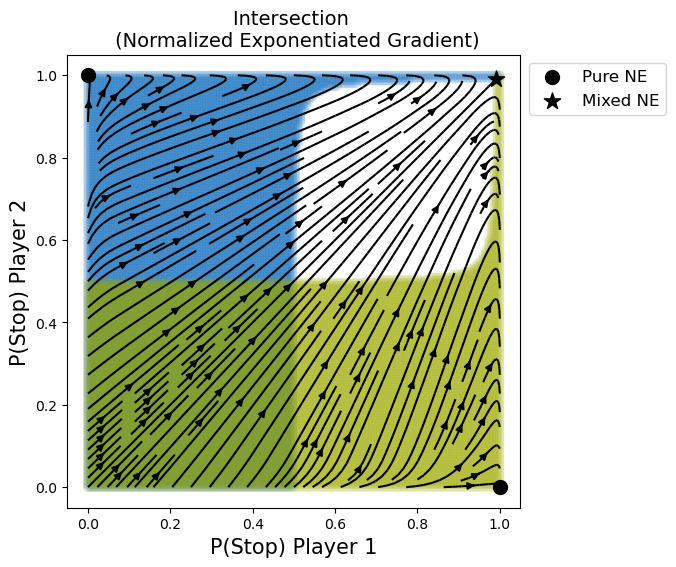
\includegraphics[width=0.5\textwidth]{logos/Intersection4.png}
    \caption{NEG vector field in the Intersection game with stable regions colored}
    \label{fig:Intersection4}
\end{figure}

Figure \ref{fig:Intersection4} might be misleading as is seems like the algorithm converges to the MNE. Even though the MNE seems to be attracting, both algorithms eventually converge to an PNE for all initial strategies except from the perfect diagonal. I have plotted a single trajectory in figure \ref{fig:Intersection5} to clarify that. 

\begin{figure}[H]
    \centering
    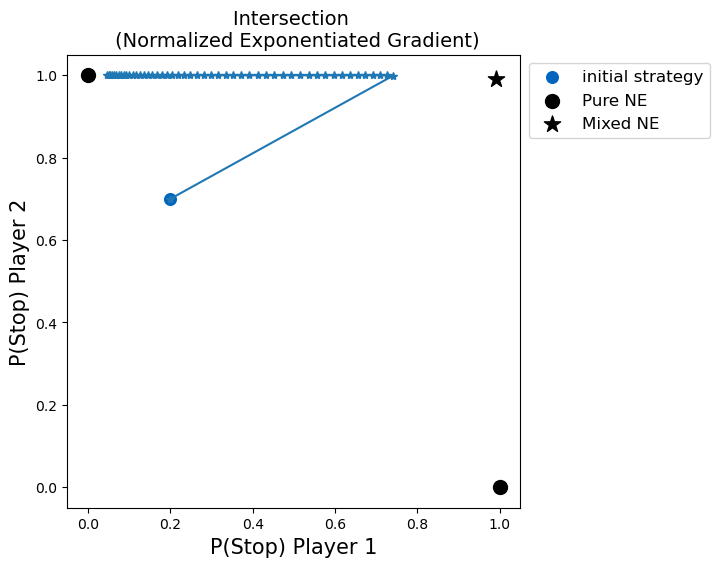
\includegraphics[width=0.5\textwidth]{logos/Intersection5.png}
    \caption{NEG single trajectory for the initial strategy $x_{1}^{0} = (0.2,0.8)$, $x_{2}^{0} = (0.7,0.3)$}
    \label{fig:Intersection5}
\end{figure}

Just like in Battle of Sexes we cannot find a neighborhood for the MNE such that the equation of the stability definition \ref{def:stability} is fulfilled. As we zoom in to the MNE again we cannot draw a circle around the MNE such that all points within the circle are colored, as illustrated in figure \ref{fig:Intersection6}. The same observations could be made for OGDLP. 

\begin{figure}[H]
    \centering
    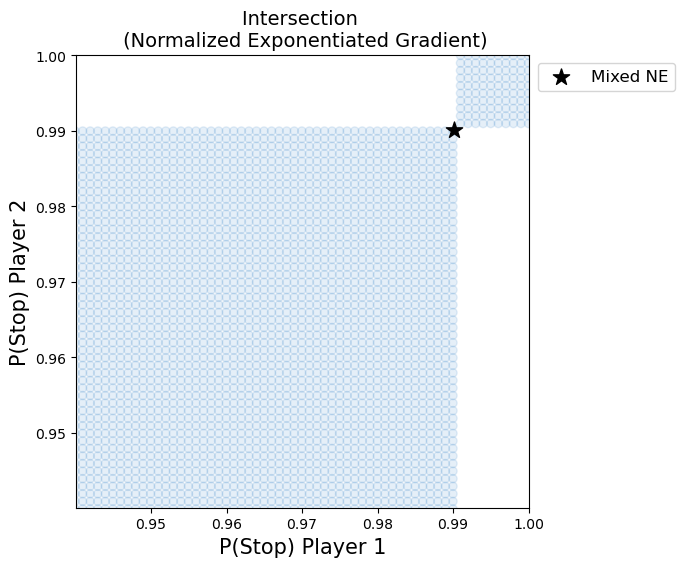
\includegraphics[width=0.5\textwidth]{logos/Intersection6.png}
    \caption{Zoomed in to the MNE in the Intersection Game}
    \label{fig:Intersection6}
\end{figure}


\subsection{Coordination Game}\label{subsection:coordinationGame}

The behaviour of the Coordination game under \textit{no-regret} dynamics has already been studied in \cite{jafari} but other \textit{no-regret} algorithms than NEG and OGDLP were used. As the name suggests, both player aim to cooperate, see table \ref{tab:payoffCoordination3x3}. 

\begin{table}[H]\centering
\setlength{\extrarowheight}{2pt}
\begin{tabular}{cc|c|c|c|}
  & \multicolumn{1}{c}{} & \multicolumn{1}{c}{$L$}  & \multicolumn{1}{c}{$C$}  & \multicolumn{1}{c}{$R$} \\\cline{3-5}
            & $T$ & $3,3$ & $0,0$ & $0,0$ \\ \cline{3-5}
            & $M$ & $0,0$ & $2,2$ & $0,0$ \\\cline{3-5}
            & $B$ & $0,0$ & $0,0$ & $1,1$ \\\cline{3-5}
\end{tabular}\caption{\label{tab:payoffCoordination3x3}payoff matrix Coordination Game}
\end{table}

There are three \textit{pure Nash equilibria} and multiple \textit{fully mixed Nash equilibria}. As we have seen in the previous examples \textit{fully mixed Nash equilibria} are not \textit{stable} therefore not learnable under \textit{no-regret} dynamics. For that reason we will neglect MNEs from now on. Lets consider the following three PNEs.

\begin{description}\centering
    \item $x^{*} = (T,L) \qquad \textit{strict }\text{PNE}$
    \item $x^{*} = (M,C) \qquad \textit{strict }\text{PNE}$
    \item $x^{*} = (B,R) \qquad \textit{strict }\text{PNE}$
\end{description}

Obviously all of them are \textit{strict} PNEs as any unilateral deviation from an PNE results in a decrease in payoff. Note that \textit{(B,R)} is \textit{pareto dominated} by \textit{(M,C)} which is once again \textit{pareto dominated} by \textit{(T,L)}, so \textit{(T,L)} is \textit{pareto optimal}. \\

One might assume that for any general-sum game that is not constant-sum \textit{no-regret} algorithms do not converge as we observed in the Shapley Game in subsection \ref{subsection:shapleyGame}. In the Coordination game however I found convergence to one of the above PNEs for all initial strategies. I have randomized the players' initail strategies and actually most of the time both algorithms converged to the \textit{pareto optimal} PNE \textit{(T,L)} (see an example in figure \ref{fig:Coordination3x3-1}). 

\begin{figure}[H]
    \centering
    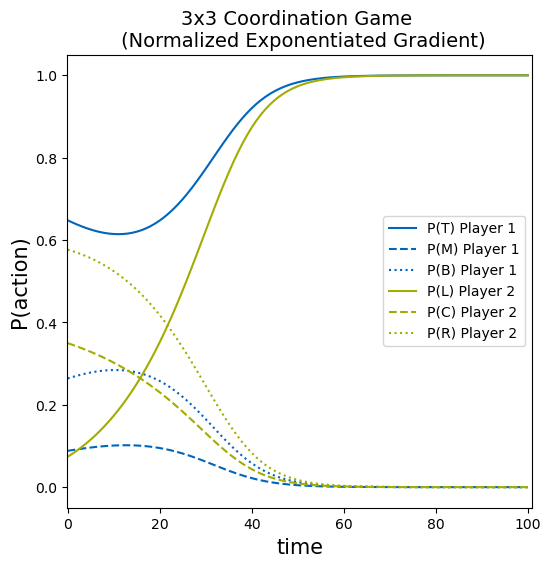
\includegraphics[width=0.5\textwidth]{logos/Coordination3x3-1.png}
    \caption{NEG convergence to the PNE \textit{(T,L)}}
    \label{fig:Coordination3x3-1}
\end{figure}

Less often I found convergence to the PNE \textit{(M,C)} (see figure \ref{fig:Coordination3x3-2}) and even less often to the PNE \textit{(B,R)} (see figure \ref{fig:Coordination3x3-3}). Unfortunately I haven't found a pattern for which initial strategy the algorithms converge to a specific PNE but the fact that most of the time it converges to \textit{(T,L)} might probably have something to do with its \textit{pareto dominance}. 

\begin{figure}[H]
    \centering
    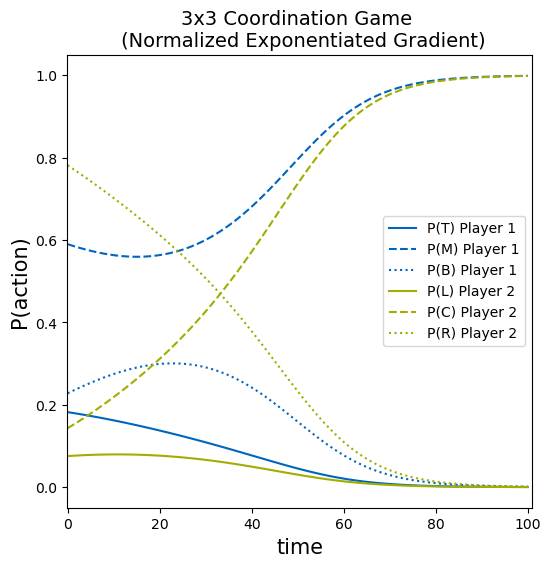
\includegraphics[width=0.5\textwidth]{logos/Coordination3x3-2.png}
    \caption{NEG convergence to the PNE \textit{(M,C)}}
    \label{fig:Coordination3x3-2}
\end{figure}

\begin{figure}[H]
    \centering
    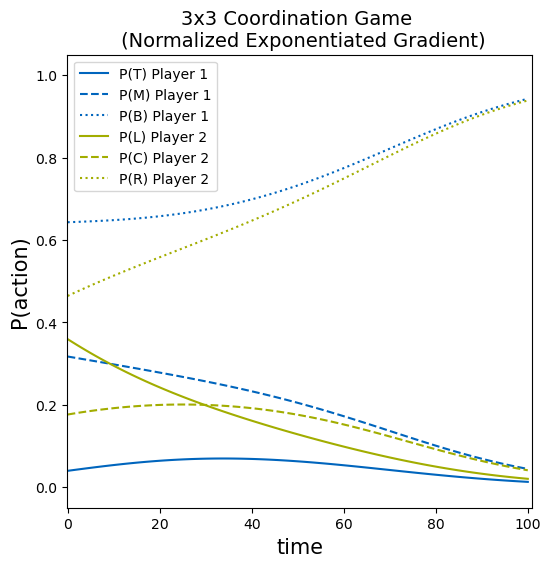
\includegraphics[width=0.5\textwidth]{logos/Coordination3x3-3.png}
    \caption{NEG convergence to the PNE \textit{(B,R)}}
    \label{fig:Coordination3x3-3}
\end{figure}

The reason why both algorithms converge to \textit{Nash equilibria} in the Coordination game and diverge in the Shapley Game is because there exists no \textit{strict} NE in the Shapley Game. As we have concluded in chapter \ref{chapter:literatureReview} only \textit{strict} NE survive under \textit{no-regret} dynamics which means in games where no \textit{strict} NE exists we need to expect that the induced sequence of play diverges, as it did in the Shapley game. Note that empirical frequency of play might still converge even though no \textit{strict} NE exists as we observed in the constant-sum games Matching Pennies and Rock Paper Scissors. 


\section{Weak Nash Equilibria}\label{section:WeakNashEquilibria}

\subsection{Strict and Weak Nash Equilibria 2x2}\label{subsection:2x2}

Lastly, I would like to address games in which both \textit{strict} and \textit{weak pure Nash equilibria} exist. Consider the 2x2 payoff matrix in table \ref{tab:payoffStrictAndWeak2x2}.

\begin{table}[H]\centering
\setlength{\extrarowheight}{2pt}
\begin{tabular}{cc|c|c|}
  & \multicolumn{1}{c}{} & \multicolumn{1}{c}{$H$}  & \multicolumn{1}{c}{$T$} \\\cline{3-4}
  & $H$ & $2,3$ & $1,2$ \\\cline{3-4}
  & $T$ & $1,2$ & $2,2$ \\\cline{3-4}
\end{tabular}\caption{\label{tab:payoffStrictAndWeak2x2}payoff matrix \textit{strict} and \textit{weak} Nash equilibria 2x2}
\end{table}

The game yields one \textit{mixed} and two \textit{pure Nash equilibria}. As the MNE is again not \textit{stable} and as expected the sequence of play for both algorithms didn't converge to the MNE we will focus on the two PNEs. 

\begin{description}\centering
    \item $x^{*} = (H,H) \qquad \textit{strict }\text{PNE}$
    \item $x^{*} = (T,T) \qquad \textit{weak }\text{PNE}$
\end{description}

Lets first look at \textit{(H,H)}. It is \textit{strict} in a sense of definition \ref{def:strictNE} as any unilateral deviation leads to a strict decrease in payoff. For instance, if the \textit{row player} expects the \textit{column player} to play \textit{H} then deviating from \textit{H} to \textit{T} would lead to a reduced payoff from $2$ to $1$. Equivalently expecting the \textit{row player} to play \textit{H}, the \textit{column player's} payoff decreses from $3$ to $2$ if the \textit{column player} deviates from \textit{H} to \textit{T}. Therefore \textit{(H,H)} is a \textit{strict} PNE. \\

\textit{(T,T)} on the other hand is \textit{weak}. A PNE is called \textit{weak} when there is no incentive for any player to unilaterally deviate but if they do they do not necessarily reduce their payoff, or equivalently there exist more than one unique best response to the PNE. In the specific game above \textit{(T,T)} is \textit{weak} because expecting the \textit{row player} to play \textit{T} the \textit{row player} can deviate from \textit{T} to \textit{H} without reducing its payoff as $2 \nless 2$. Note that \textit{(T,T)} is still an PNE as the payoff also doesn't strictly increase when deviating. \\

Now I would like to validate the result from chapter \ref{chapter:literatureReview} that only \textit{strict} PNE survive under \textit{no-regret} dynamics. First of all the \textit{weak} PNE \textit{(T,T)} is not \textit{stable} in a sense of definition \ref{def:stability}. There are always strategies in the neighborhood of the \textit{weak PNE} that did not fulfill the definition. Especially strategies profile where the \textit{row player} played \textit{T} with probability $1$ and \textit{H} with probability $0$ I found gaps that were not \textit{stable} with respect to the \textit{weak} PNE no matter how much we zoom in, see figure \ref{fig:Weak1}. Blue points are strategy profiles for which the stability definition holds. This observations fits proposition \ref{prop:StrictStableEquivalent} saying that only \textit{strict} PNEs are \textit{stable}.

\begin{figure}[H]
    \centering
    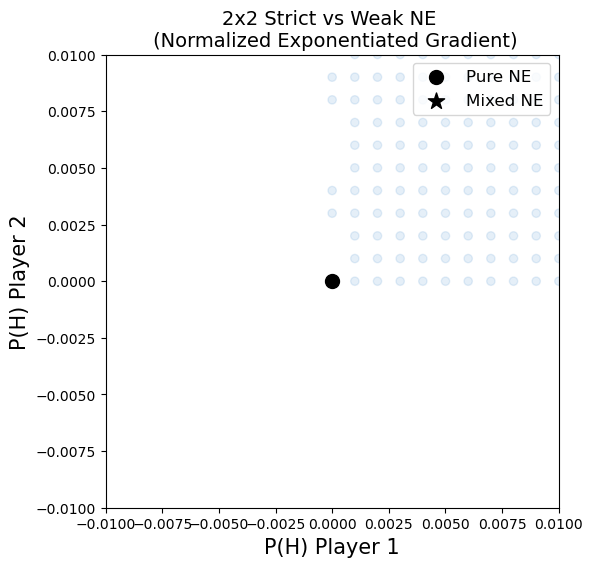
\includegraphics[width=0.5\textwidth]{logos/Weak1.png}
    \caption{Zoomed in to the \textit{weak} PNE}
    \label{fig:Weak1}
\end{figure}

For the \textit{strict} PNE \textit{(H,H)} I found \textit{local stability} as depicted by the blue region in figure \ref{fig:Weak2}. 

\begin{figure}[H]
    \centering
    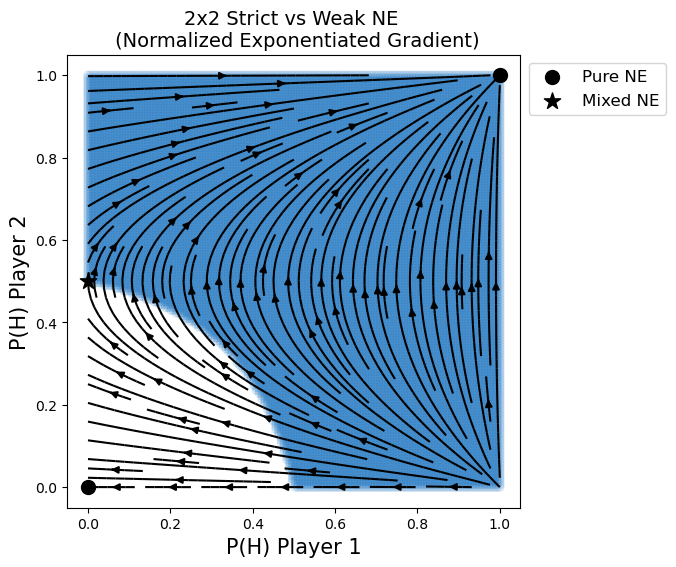
\includegraphics[width=0.5\textwidth]{logos/Weak2.png}
    \caption{NEG vector field in 2x2 \textit{strict} and \textit{weak Nash equilibira}}
    \label{fig:Weak2}
\end{figure}

The figure might be misleading though as it looks like the NEG algorithm steps outside the feasible probability simplex. A closer examination however showed that for some initial strategies that are locally close to the \textit{weak} PNE the NEG algorithm diverges towards the "left wall". An example trajectory for that phenomena is shown in figure \ref{fig:Weak4}.

\begin{figure}[H]
    \centering
    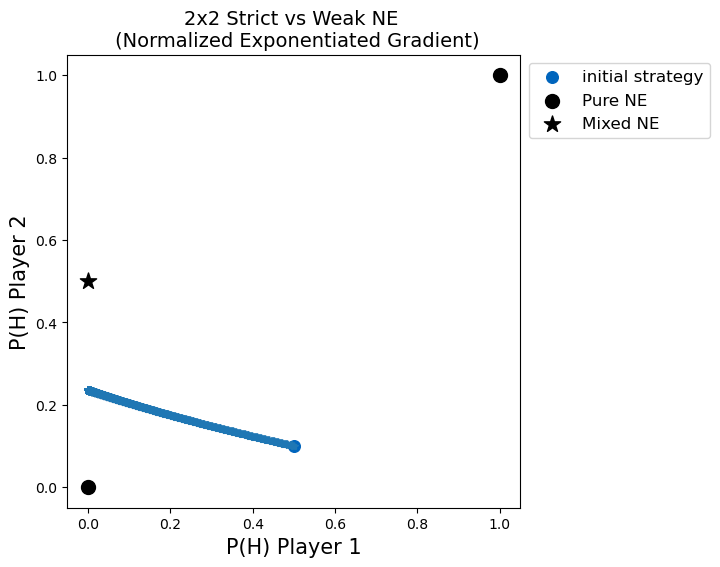
\includegraphics[width=0.5\textwidth]{logos/Weak4.png}
    \caption{NEG single trajectory for the initial strategy $x_{1}^{0} = (0.5,0.5)$, $x_{2}^{0} = (0.1,0.9)$}
    \label{fig:Weak4}
\end{figure}

No matter how much iterations were used, the NEG algorithm didn't change its direction. Changing the initial strategy slightly closer towards the \textit{strict} PNE, however, yields convergence as illustrated in \ref{fig:Weak3}. 

\begin{figure}[H]
    \centering
    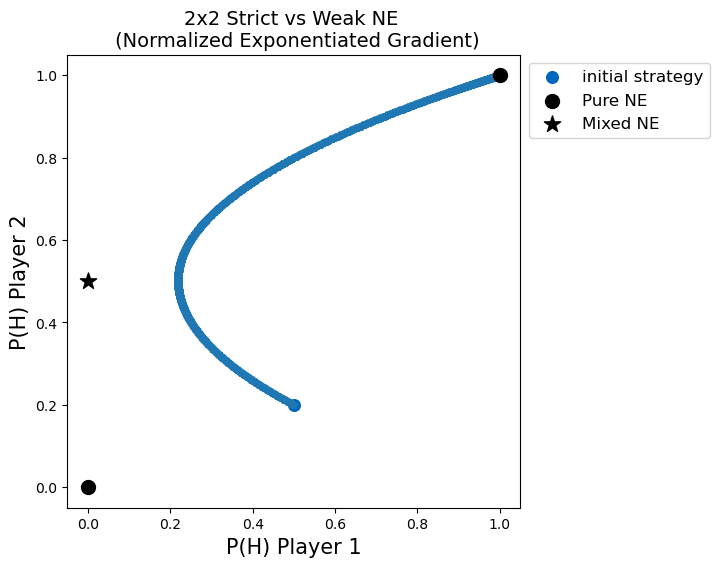
\includegraphics[width=0.5\textwidth]{logos/Weak3.png}
    \caption{NEG single trajectory for the initial strategy $x_{1}^{0} = (0.5,0.5)$, $x_{2}^{0} = (0.2,0.8)$}
    \label{fig:Weak3}
\end{figure}

So indeed the \textit{strict} and therefore \textit{stable} PNE is also locally attracting (proposition \ref{prop:localConvergence}). But even though there exists a unique \textit{strict} PNE, as in the Prisoner's Dilemma, this game shows that \textit{no-regret} dynamics do not converge to it globally. It seems like the existence of a \textit{weak} PNE is disrupting the convergence to the \textit{strict} PNE. Also its worth mentioning that for no inital strategy I have found convergence to the \textit{weak} PNE but rather divergence towards the "left wall". I came to the same conclusions for the OGDLP algorithm, see figure \ref{fig:Weak5}

\begin{figure}[H]
    \centering
    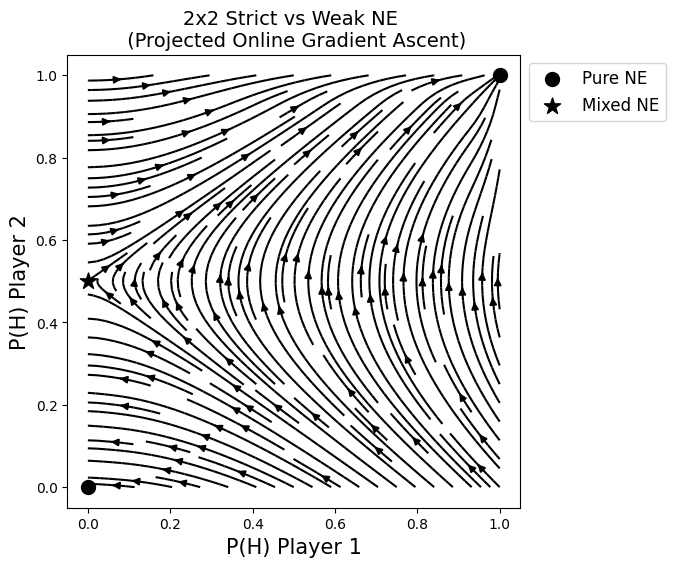
\includegraphics[width=0.5\textwidth]{logos/Weak5.png}
    \caption{OGDLP vector field in 2x2 \textit{strict} and \textit{weak Nash equilibira}}
    \label{fig:Weak5}
\end{figure}


\subsection{Strict and Weak Nash Equilibria 3x3}\label{subsection:3x3}

The following game is a 3x3 general-sum game that has two \textit{strict} and one \textit{weak pure Nash equilibria}. There are also multiple \textit{fully mixed Nash equilibria} but they are negelected again as the sequence of play never converges to one of them for the very same reason that interior states cannot be \textit{stable} and therefore not attracting under \textit{no-regret} dynamics (proposition \ref{prop:noInteriorStable}). Consider the 3x3 payoff matrix described in table \ref{tab:payoffStrictAndWeak3x3}. 

\begin{table}[H]\centering
\setlength{\extrarowheight}{2pt}
\begin{tabular}{cc|c|c|c|}
  & \multicolumn{1}{c}{} & \multicolumn{1}{c}{$A$}  & \multicolumn{1}{c}{$B$}  & \multicolumn{1}{c}{$C$} \\\cline{3-5}
            & $X$ & $2,3$ & $1,2$ & $1,1$ \\ \cline{3-5}
            & $Y$ & $1,1$ & $2,1$ & $3,2$ \\\cline{3-5}
            & $Z$ & $1,2$ & $2,2$ & $2,1$ \\\cline{3-5}
\end{tabular}\caption{\label{tab:payoffStrictAndWeak3x3}payoff matrix \textit{strict} and \textit{weak} Nash equilibria 3x3}
\end{table}

The three \textit{pure Nash equilibria} are

\begin{description}\centering
    \item $x^{*} = (X,A) \qquad \textit{strict }\text{PNE}$
    \item $x^{*} = (Y,C) \qquad \textit{strict }\text{PNE}$
    \item $x^{*} = (Z,B) \qquad \textit{weak }\text{PNE}$
\end{description}

One can easily check that \textit{(X,A)} and \textit{(Y,B)} are \textit{strict} as they are unique best responses. \textit{(Z,B)} however is not a unique best response for the \textit{column player}. Assuming the \textit{row player} to choose \textit{Z}, the \textit{column player} can deviate from \textit{B} to \textit{A} without loosing any payoff. The payoff for the \textit{column player} stays at $2$ for that deviation. Therefore \textit{(Z,B)} is \textit{weak}. \\

As far as convergence is concerned I found similar result as in the 2x2 game discussed previously. The initial strategies were randomized. In every case I found convergence of both NEG and OGDLP to one of the \textit{strict} PNE. Table \ref{fig:Weak3x3-1} shows an example for convergence to \textit{(X,A)}. Less often I found convergence to the other \textit{strict} PNE \textit{(Y,B)}, see an example in table \ref{fig:Weak3x3-2}. 

\begin{figure}[H]
    \centering
    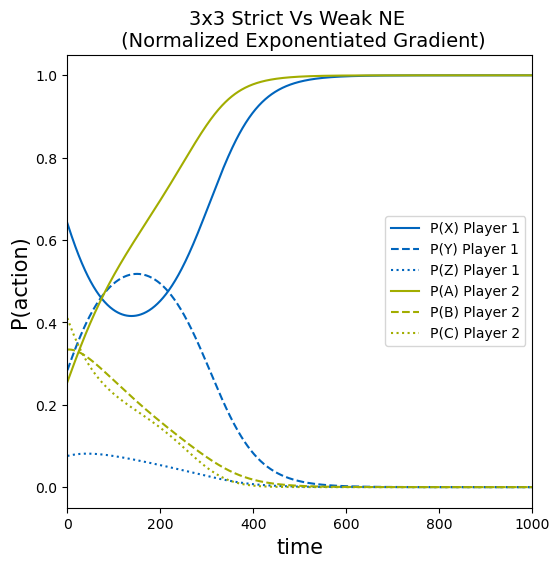
\includegraphics[width=0.5\textwidth]{logos/Weak3x3-1.png}
    \caption{NEG convergence to the \textit{strict }PNE \textit{(X,A)}}
    \label{fig:Weak3x3-1}
\end{figure}

\begin{figure}[H]
    \centering
    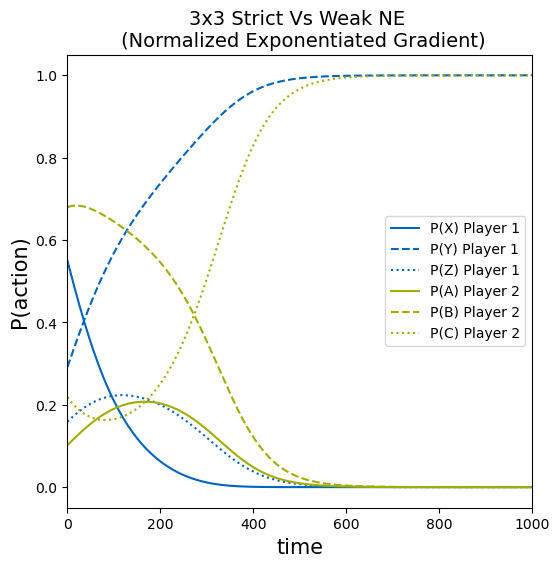
\includegraphics[width=0.5\textwidth]{logos/Weak3x3-2.png}
    \caption{NEG convergence to the \textit{strict }PNE \textit{(Y,B)}}
    \label{fig:Weak3x3-2}
\end{figure}

For non of the tested initial strategy profiles I found convergence to neither the \textit{weak} PNE \textit{(Z,B)} nor any of the \textit{fully mixed} NE. Again these empirical findings match the general result that under \textit{no-regret} dynamics only \textit{strict Nash equilibria} survive.  
